\documentclass [11pt, a4wide, twoside]{article}

\usepackage{times}
\usepackage{epsfig}
\usepackage{ifthen}
\usepackage{xspace}
\usepackage{fancyhdr}
\usepackage[colorlinks = true,linkcolor = black,urlcolor  = blue,citecolor = black,anchorcolor = black]{hyperref}
\usepackage{verbatim}
\usepackage{amsmath}
\usepackage{graphicx}

\usepackage{listings}
\usepackage{color}

\usepackage{amsmath}
\usepackage{float}

\definecolor{dkgreen}{rgb}{0,0.6,0}
\definecolor{gray}{rgb}{0.5,0.5,0.5}
\definecolor{mauve}{rgb}{0.58,0,0.82}

\lstset{frame=tb,
  language=Java,
  aboveskip=3mm,
  belowskip=3mm,
  showstringspaces=false,
  columns=flexible,
  basicstyle={\small\ttfamily},
  numbers=none,
  numberstyle=\tiny\color{gray},
  keywordstyle=\color{blue},
  commentstyle=\color{dkgreen},
  stringstyle=\color{mauve},
  breaklines=true,
  breakatwhitespace=true
  tabsize=3
}

\newboolean{showsolution}
\setboolean{showsolution}{true} 

\usepackage{times}
\usepackage{epsfig}
\usepackage{ifthen}
\usepackage{xspace}
\usepackage{fancyhdr}
\usepackage{amsthm}
\usepackage{hyperref}



%layout
\topmargin      -5.0mm
\oddsidemargin  6.0mm
\evensidemargin -6.0mm
\textheight     215.5mm
\textwidth      160.0mm
\parindent      1.0em
\headsep        10.3mm
\headheight     12pt
\lineskip       1pt
\normallineskip 1pt

\newtheorem{mydef}{Definition}


%header
\lhead{Software Modeling and Analysis \\ 2016}

\rhead{Prof. Oscar Nierstrasz, Mohammad Ghafari, Nevena Milojkovi\'{c} and Yuriy Tymchuk}

\lfoot{page \thepage}
\rfoot{\today}
\cfoot{}

\renewcommand{\headrulewidth}{0.1pt}
\renewcommand{\footrulewidth}{0.1pt}

%enumeration
\newenvironment{myitemize}{%
     \begin{itemize}
     \setlength{\itemsep}{0cm}}
     {\end{itemize}}

\newenvironment{myenumerate}{%
     \begin{enumerate} \setlength{\itemsep}{0cm}}
     {\end{enumerate}}


%solution
\ifthenelse{\boolean{showsolution}}
   {  \newcommand{\solution}[1]{
   	\noindent\underline{\textbf{Answer:}}\\[2mm]
   	 \textsl{#1}
	 \vspace{10pt}
	 \normalsize
	}
  }
  {  \newcommand{\solution}[1]{} }


\pagestyle{fancy}

% ============================================================
% Markup macros for proof-reading
\usepackage{ifthen}
\usepackage[normalem]{ulem} % for \sout
\usepackage{xcolor}
\newcommand{\ra}{$\rightarrow$}
\newboolean{showedits}
\setboolean{showedits}{true} % toggle to show or hide edits
\ifthenelse{\boolean{showedits}}
{
	\newcommand{\ugh}[1]{\textcolor{red}{\uwave{#1}}} % please rephrase
	\newcommand{\ins}[1]{\textcolor{blue}{\uline{#1}}} % please insert
	\newcommand{\del}[1]{\textcolor{red}{\sout{#1}}} % please delete
	\newcommand{\chg}[2]{\textcolor{red}{\sout{#1}}{\ra}\textcolor{blue}{\uline{#2}}} % please change
}{
	\newcommand{\ugh}[1]{#1} % please rephrase
	\newcommand{\ins}[1]{#1} % please insert
	\newcommand{\del}[1]{} % please delete
	\newcommand{\chg}[2]{#2}
}
% ============================================================
% Put edit comments in a really ugly standout display
%\usepackage{ifthen}
\usepackage{amssymb}
\newboolean{showcomments}
\setboolean{showcomments}{true}
%\setboolean{showcomments}{false}
\newcommand{\id}[1]{$-$Id: scgPaper.tex 32478 2010-04-29 09:11:32Z oscar $-$}
\newcommand{\yellowbox}[1]{\fcolorbox{gray}{yellow}{\bfseries\sffamily\scriptsize#1}}
\newcommand{\triangles}[1]{{\sf\small$\blacktriangleright$\textit{#1}$\blacktriangleleft$}}
\ifthenelse{\boolean{showcomments}}
%{\newcommand{\nb}[2]{{\yellowbox{#1}\triangles{#2}}}
{\newcommand{\nbc}[3]{
 {\colorbox{#3}{\bfseries\sffamily\scriptsize\textcolor{white}{#1}}}
 {\textcolor{#3}{\sf\small$\blacktriangleright$\textit{#2}$\blacktriangleleft$}}}
 \newcommand{\version}{\emph{\scriptsize\id}}}
{\newcommand{\nbc}[3]{}
 \renewcommand{\ugh}[1]{#1} % please rephrase
 \renewcommand{\ins}[1]{#1} % please insert
 \renewcommand{\del}[1]{} % please delete
 \renewcommand{\chg}[2]{#2} % please change
 \newcommand{\version}{}}
\newcommand{\nb}[2]{\nbc{#1}{#2}{orange}}
\newcommand{\here}{\yellowbox{$\Rightarrow$ CONTINUE HERE $\Leftarrow$}}
\newcommand\rev[2]{\nb{TODO (rev #1)}{#2}} % reviewer comments
\newcommand\fix[1]{\nb{FIX}{#1}}
\newcommand\todo[1]{\nb{TO DO}{#1}}
\newcommand\on[1]{\nbc{ON}{#1}{red}} % add more author macros here
%\newcommand\XXX[1]{\nbc{XXX}{#1}{blue}}
%\newcommand\XXX[1]{\nbc{XXX}{#1}{brown}}
%\newcommand\XXX[1]{\nbc{XXX}{#1}{cyan}}
%\newcommand\XXX[1]{\nbc{XXX}{#1}{darkgray}}
%\newcommand\XXX[1]{\nbc{XXX}{#1}{gray}}
%\newcommand\XXX[1]{\nbc{XXX}{#1}{magenta}}
%\newcommand\XXX[1]{\nbc{XXX}{#1}{olive}}
%\newcommand\XXX[1]{\nbc{XXX}{#1}{orange}}
%\newcommand\XXX[1]{\nbc{XXX}{#1}{purple}}
%\newcommand\XXX[1]{\nbc{XXX}{#1}{red}}
%\newcommand\XXX[1]{\nbc{XXX}{#1}{teal}}
%\newcommand\XXX[1]{\nbc{XXX}{#1}{violet}}
%=============================================================
% ST80 listings macros
% Adapted from Squeak by Example book
%=============================================================
% If you want >>> appearing as right guillemet, you need these two lines:
%\usepackage[T1]{fontenc}
%\newcommand{\sep}{\mbox{>>}}
% Otherwise use this:
\newcommand{\sep}{\mbox{$\gg$}}
%=============================================================
%:\needlines{N} before code block to force page feed
\usepackage{needspace}
\newcommand{\needlines}[1]{\Needspace{#1\baselineskip}}
%=============================================================
%:Listings package configuration for ST80
\usepackage[english]{babel}
\usepackage{amssymb,textcomp}
\usepackage{listings}
% \usepackage[usenames,dvipsnames]{color}
% \usepackage[usenames]{color}
% \definecolor{source}{gray}{0.95}
\lstdefinelanguage{Smalltalk}{
%  morekeywords={self,super,true,false,nil,thisContext}, % This is overkill
  morestring=[d]',
  morecomment=[s]{"}{"},
  alsoletter={\#:},
  escapechar={!},
  literate=
    {BANG}{!}1
    {UNDERSCORE}{\_}1
    {\\st}{Smalltalk}9 % convenience -- in case \st occurs in code
    % {'}{{\textquotesingle}}1 % replaced by upquote=true in \lstset
    {_}{{$\leftarrow$}}1
    {>>>}{{\sep}}1
    {^}{{$\uparrow$}}1
    {~}{{$\sim$}}1
    {-}{{\sf -\hspace{-0.13em}-}}1  % the goal is to make - the same width as +
    {+}{\raisebox{0.08ex}{+}}1		% and to raise + off the baseline to match -
    {-->}{{\quad$\longrightarrow$\quad}}3
	, % Don't forget the comma at the end!
  tabsize=4
}[keywords,comments,strings]

\definecolor{source}{gray}{0.95}

\lstset{language=Smalltalk,
	basicstyle=\sffamily,
	keywordstyle=\color{black}\bfseries,
	% stringstyle=\ttfamily, % Ugly! do we really want this? -- on
	mathescape=true,
	showstringspaces=false,
	keepspaces=true,
	breaklines=true,
	breakautoindent=true,
	backgroundcolor=\color{source},
	lineskip={-1pt}, % Ugly hack
	upquote=true, % straight quote; requires textcomp package
	columns=fullflexible} % no fixed width fonts
% In-line code (literal)
% Normally use this for all in-line code:
\newcommand{\ct}{\lstinline[mathescape=false,backgroundcolor=\color{white},basicstyle={\sffamily\upshape}]}
% In-line code (latex enabled)
% Use this only in special situations where \ct does not work
% (within section headings ...):
\newcommand{\lct}[1]{{\textsf{\textup{#1}}}}
% Code environments
\lstnewenvironment{code}{%
	\lstset{%
		% frame=lines,
		frame=single,
		framerule=0pt,
		mathescape=false
	}
}{}

% Useful to add a matching $ after code containing a $
% \def\ignoredollar#1{}
%=============================================================
\newcommand{\ie}{\emph{i.e.}\xspace}
\newcommand{\eg}{\emph{e.g.}\xspace}
\newcommand{\etal}{\emph{et al.}\xspace}
% ============================================================

\definecolor{mircolor}{rgb}{0.4,0.6,0.2}
\newcommand\ml[1]{\nbc{ML}{#1}{mircolor}}
%\usepackage{wasysym}
\newcommand\yesml[1]{\nbc{ML {\textcolor{yellow}\sun}}{#1}{mircolor}}

\begin{document}

\section*{\ifthenelse{\boolean{showsolution}}{\textcolor{red}{Solution}\\}{}Assignment 06 --- 21.10.2020 -- v1.0\\Software Visualization}

\textcolor{red}{Please submit this exercise by email to \href{mailto:pascal.gadient@inf.unibe.ch}{pascal.gadient@inf.unibe.ch} \underline{before} 28 October 2020, 10:15am.\begin{center}\textbf{You must submit your code as editable text, i.e., use plain text file(s).}\end{center}}

\noindent For this assignment, we need Pharo 9.0 (instead of the previous 8.0 releases). If not already done, download the latest \underline{stand-alone} release of \emph{Pharo Launcher} from \href{https://pharo.org/download}{here} and install the application. After it is successfully installed, start the application and click on ``New'' (top left). In the new window that appears, choose ``Official distributions'' and ``Pharo 9.0 - 64bit (development version, latest)'' (or the corresponding 32bit release if your CPU or OS does not support 64 bits). Click on ``Create image''. Select the newly created \emph{Pharo} entry from the list and click on ``Launch''. A new window that runs Pharo will be displayed.\\\\
Next, we have to enable additional feature support in Roassal3, e.g., for the method \texttt{number\-Of\-Lines\-Of\-Code}. For that, in the main screen of Pharo 9.0 click on the menu ``Tools'', then ``Roassal3'', and finally on ``Load full version''. This process can take several minutes depending on your device's CPU and internet connection. We advise you to save the image when the installation succeeded to avoid redoing this process.\\\\
Your task is to create plots that look as similar as possible to those presented in each exercise, including the colors and spacings.\\\\\\
Troubleshooting:
\begin{enumerate}
\item Problem (macOS only):\\Launcher won't launch.\\\\
Solution:\\Change the launcher setting to launch with login shell (query ``login'' in the settings and uncheck ``Launch image from a login shell'')
\item Problem (macOS only):\\
Launcher won't launch.\\\\
Solution:\\Acknowledge the dialog where the app asks for trust.
\end{enumerate}


%\textit{NB: For the following exercises we use the \emph{Roassal3} environment \href{https://github.com/ObjectProfile/Roassal3}{available on Github}. You can download and install Roassal3 automatically in your GT environment by executing the statement below in the Playground.\\\\
%\texttt{Metacello new\\
%\hspace*{0.5cm}baseline: \textquotesingle Roassal3\textquotesingle;\\
% \hspace*{0.5cm}repository: \textquotesingle github://ObjectProfile/Roassal3:v0.9.5\textquotesingle;\\
% \hspace*{0.5cm}load.}\\\\
% Be warned: it can take 15 minutes or more to download and install within GT. During that time GT remains unresponsive to any user input. We advise you to save the image as soon as the installation succeeded to avoid redoing this process.}

\newpage

\subsection*{Exercise 1: Sunburst visualization with Roassal (2 pts)}
Build a Sunburst visualization as shown in \autoref{fig:sunburst} to analyze the test coverage of the \texttt{Collection} class hierarchy. Each tile represents a specific class, and the size of the tile should represent its number of lines of code. Moreover, tested classes (i.e., classes covered by tests) should be colored in green, while other classes should remain in grey.\\\\
Hint: You can assume that test classes (i.e., classes that test other classes) use a name which closely resembles the original name of the class they test; in general, they add only the postfix \texttt{Test} to the original class name (e.g., \texttt{ByteArray} will become to \texttt{ByteArrayTest}).\\

\begin{figure}[H]
\centering
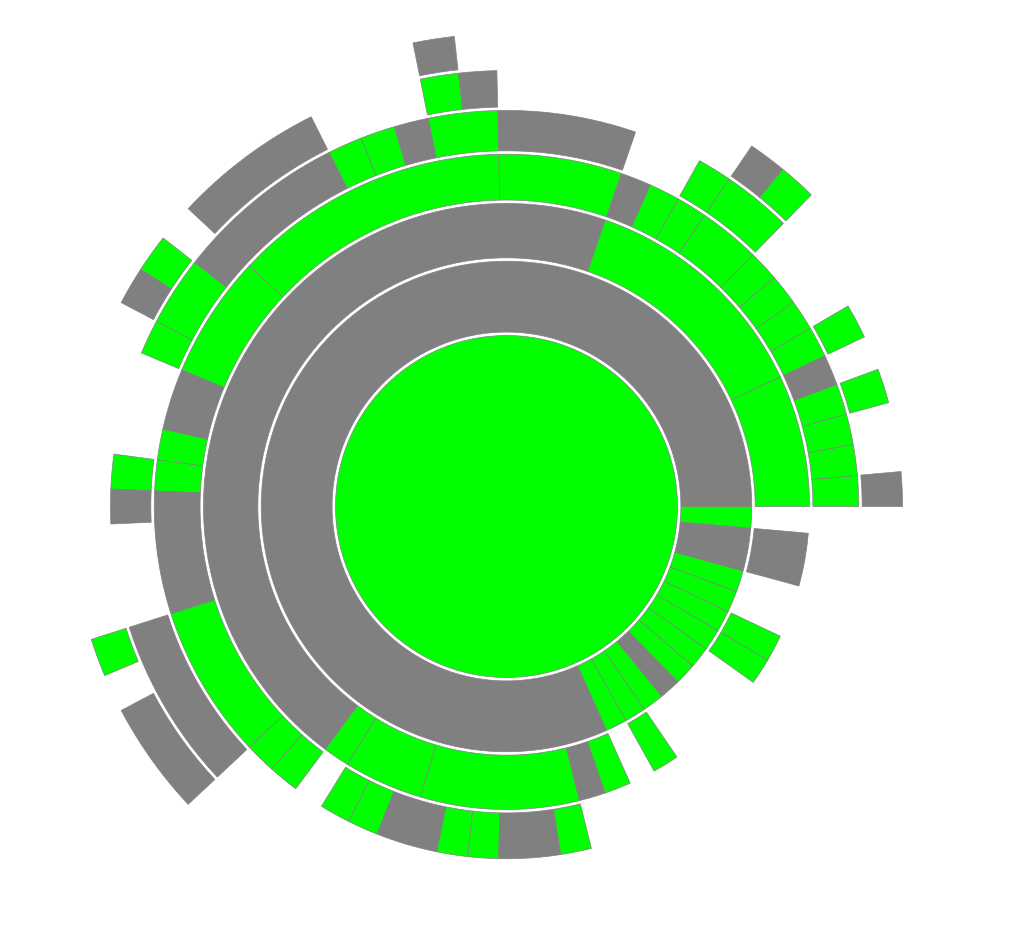
\includegraphics[scale=0.5]{images/1.png}
\caption{Sunburst visualization built with Roassal}
\label{fig:sunburst}
\end{figure}


\ifthenelse{\boolean{showsolution}}{\newpage}{}

\solution{\noindent \texttt{\textbar~sb \textbar\\
sb := RSSunburstBuilder new.\\
sb sliceShape withBorder.\\
sb sliceColor: [:shape \textbar\\
\hspace*{0.5cm}(Smalltalk includesKey: (shape model name , \textquotesingle Test\textquotesingle) asSymbol)\\
\hspace*{0.5cm}ifTrue: [ Color green ]\\
\hspace*{0.5cm}ifFalse: [ Color gray ] ].\\
sb explore: Collection using:  \#subclasses.\\
RSNormalizer size\\
\hspace*{0.5cm}shapes: (sb shapes select: \#isSLeaf);\\
\hspace*{0.5cm}normalize: \#numberOfLinesOfCode.\\
sb build.\\
sb canvas @ RSCanvasController.\\
\caret~sb canvas}}

\newpage

\subsection*{Exercise 2: Tree layout visualization with Roassal  (2 pts)}
Build a tree as shown in \autoref{fig:treemap} to highlight subclasses of the class \texttt{Collection}, which have again subclasses and contain the string \texttt{Array} in their names. Circles should be used to represent the classes, and the size of each circle should encode the number of methods of the represented class. Moreover, classes that have subclasses and contain the string \texttt{Array} in their names must be colored green, whereas other classes must remain grey.

\begin{figure}[H]
\centering
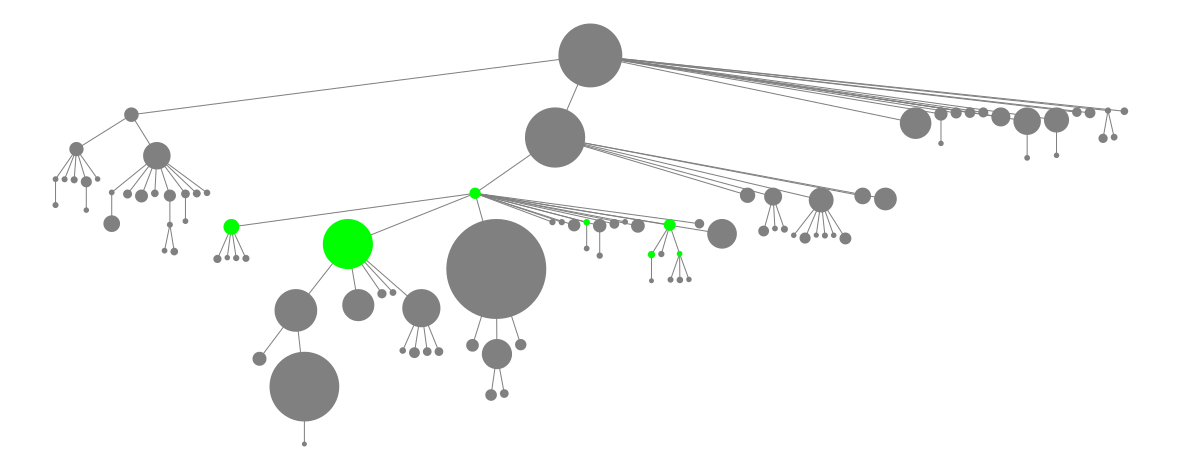
\includegraphics[scale=0.5]{images/2.png}
\caption{Tree layout visualization built with Roassal}
\label{fig:treemap}
\end{figure}

\ifthenelse{\boolean{showsolution}}{\newpage}{}

\solution{\texttt{\textbar~canvas shapes \textbar\\
canvas := RSCanvas new.\\
shapes := (Collection withAllSubclasses ) collect: [ :class \textbar\\
\hspace*{0.5cm}(class subclasses notEmpty and: [\textquotesingle *Array*\textquotesingle~match: class name])\\
\hspace*{0.5cm}ifTrue: [RSEllipse new model: class; color: Color green; popup ]\\
\hspace*{0.5cm}ifFalse: [RSEllipse new model: class; color: Color gray; popup ]].\\
canvas addAll: shapes.\\
RSEdgeBuilder line \\
\hspace*{0.5cm}canvas: canvas;\\
\hspace*{0.5cm}connectFrom: [ :class \textbar~class superclass ].\\
RSNormalizer size\\
\hspace*{0.5cm}shapes: shapes;\\
\hspace*{0.5cm}normalize: [ :cls \textbar~cls numberOfMethods].\\
RSTreeLayout on: shapes.\\
canvas edges pushBack.\\
canvas zoomToFit.\\
\caret~canvas}}

\newpage

\subsection*{Exercise 3: Node-link visualization with Roassal (3 pts)}
In this exercise you have to create a node-link visualization as shown in \autoref{fig:node-link} to analyze the class dependencies between the \texttt{Collection} class hierarchy and the \texttt{RSLayout} class hierarchy. To this end, you have to:
\begin{enumerate}[i)]
\item Visualize the classes of both hierarchies using circles (i.e., \texttt{RSEllipse})
\item Use the red (\texttt{Collection}) and green (\texttt{RSLayout}) color to highlight the classes of each hierarchy.
\item Add edges to depict the class hierarchy, while using the \texttt{RSClusterLayout}
\item Add blue Bézier edges to depict class dependencies using \texttt{RSMultiBezierEdgeBuilder}
\item Map the number of methods of each class to its circle size using \texttt{RSNormalizer}
\end{enumerate}
%Provide the Roassal code to implement such a visualization, and use it to identify the classes in each hierarchy that have the highest number of dependencies.\\

\begin{figure}[H]
\centering
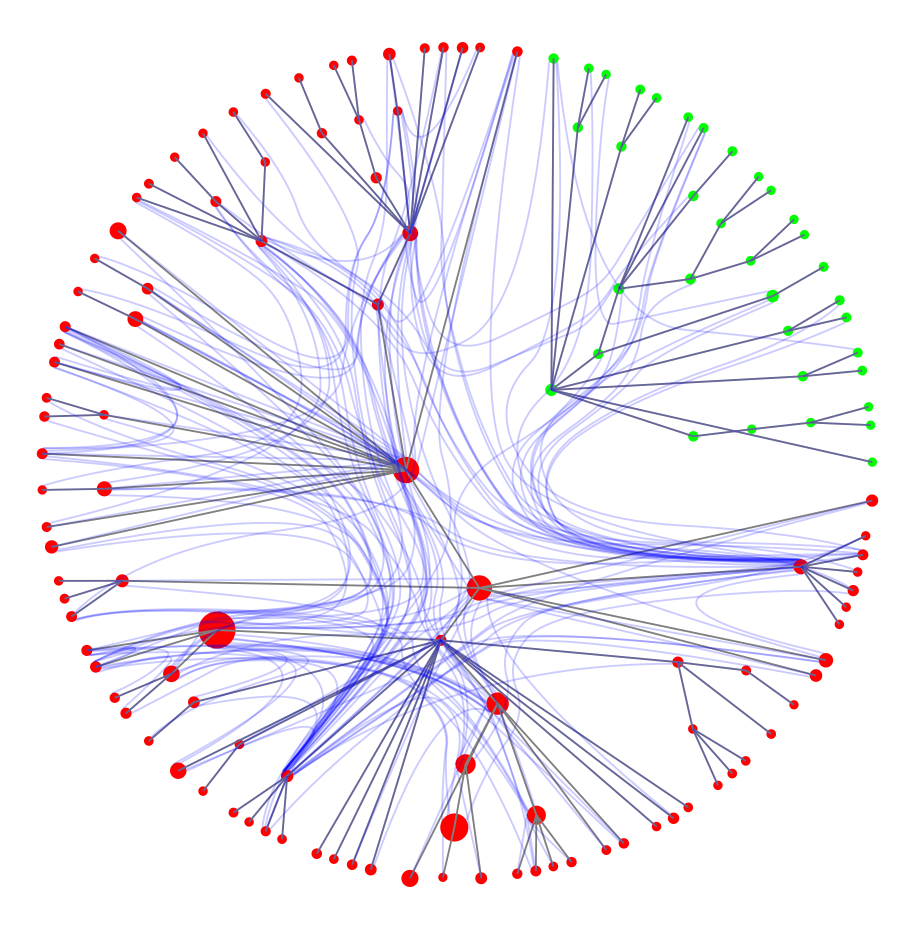
\includegraphics[scale=0.5]{images/3.png}
\caption{Node-link visualization built with Roassal}
\label{fig:node-link}
\end{figure}

\ifthenelse{\boolean{showsolution}}{\newpage}{}

\solution{\texttt{\textbar~c classes \textbar\\
c := RSCanvas new.\\
classes := RSLayout withAllSubclasses , Collection withAllSubclasses.\\
classes := classes asSet \\
\hspace*{0.5cm}collect: [ :cls \textbar~(RSLayout withAllSubclasses includes: cls)\\
\hspace*{1.0cm}ifTrue: [RSEllipse new model: cls; color: Color green] \\
\hspace*{1.0cm}ifFalse: [RSEllipse new model: cls; color: Color red]]  \\
\hspace*{0.5cm}as: RSGroup.\\
c addAll: classes.\\
RSEdgeBuilder line\\
\hspace*{0.5cm}color: Color gray;\\
\hspace*{0.5cm}canvas: c;\\
\hspace*{0.5cm}shapes: classes;\\
\hspace*{0.5cm}connectFrom: \#superclass.\\
RSNormalizer size\\
\hspace*{0.5cm}shapes: classes;\\
\hspace*{0.5cm}to: 20;\\
\hspace*{0.5cm}normalize: \#numberOfMethods.\\
RSClusterLayout on: classes.\\
RSMultiBezierEdgeBuilder multiBezier\\
\hspace*{0.5cm}borderColor: (Color blue alpha: 0.2);\\
\hspace*{0.5cm}canvas: c;\\
\hspace*{0.5cm}shapes: classes;\\
\hspace*{0.5cm}withBorderAttachPoint;\\
\hspace*{0.5cm}following: \#superclass;\\
\hspace*{0.5cm}connectToAll: \#dependentClasses.\\
c @ RSCanvasController.\\
classes @ RSPopup.\\
\caret~c}}

\ifthenelse{\boolean{showsolution}}{\newpage}{\newpage}

\subsection*{Exercise 4: Discussion (3 pts)}
Comment on the strenghts and limitations of each visualization you just created.\\
\solution{\textbf{Sunburst visualization.} The sunburst visualization provides a nice representation for hierarchies; each ring from the center moving outwards corresponds to a level in the hierarchy. The rings are sliced into numerous tiles, each of them revealing the relationship to the parent tile. Besides those advantages, anything related to the covered area of specific tiles is hard to evaluate manually, since humans cannot accurately estimate areas of circular sections.\\\\
\textbf{Tree layout visualization.} The tree layout visualization uses more space and is not as compact as
the Sunburst visualization. This effect requires more navigation. However, it is easier to analyze the
classes, relationships, and classes at the various levels in the hierarchy.\\\\
\textbf{Node-link visualization.} Node-link visualizations combine the best of both worlds: they support multiple overlaid relation visualizations (in our example using Bézier curves and straight lines) and represent the hierarchy level of each element in an intuitive manner. Unfortunately, these plots require a very high resolution to be of any use, because of their heavy utilization of tiny connections between the different shapes.}

\end{document}

